\documentclass{scrartcl}
\usepackage{listings}
\usepackage{tikz}
\lstset{basicstyle=\ttfamily,columns=flexible}
\usetikzlibrary{fit,tikzmark}
\usetikzmarklibrary{listings}
\tikzset{
  balloon/.style={
    draw,
    fill=blue!20,
    opacity=0.4,
    inner sep=4pt,
    rounded corners=2pt,
    minimum height=15pt
  },
}




\begin{document}

\begin{lstlisting}[name=OBJR]
%Link Object
18 0 obj
<< /Type /Annot
 /StructParent 16
 /Rect [ 196.109 494.573 399.167 506.831 ]
 /Subtype/Link/
 A<</Type/Action /S/URI /URI(https://github.com/u-fischer/tagpdf) >>
 >>
endobj

%Object reference (OBJR)
19 0 obj
<</Type /OBJR /Obj 18 0 R>>
endobj

%Structure Element
17 0 obj
<< /Type /StructElem /S /Link /P 11 0 R
/K [<</Type /MCR /Pg 8 0 R /MCID 6>>
    19 0 R]>>
endobj};

%Parenttree
5 0 obj
<< /Nums [...
16 17 0 R
...] >>
endobj
\end{lstlisting}
\NewDocumentCommand\balloon{O{0pt} O{0pt} m m}{%
\node[fit={([xshift=#1]pic cs:line-OBJR-#4-first) ([xshift=#2]pic cs:line-OBJR-#4-end)
([yshift=6pt,xshift=#2]pic cs:line-OBJR-#4-end)},balloon](#4balloon){};}

\begin{tikzpicture}[overlay,remember picture]
\coordinate(link)at ([xshift=3em]pic cs:line-OBJR-2-start);
\balloon{link}{2}
\coordinate(structparent) at (pic cs:line-OBJR-4-end);
\balloon{structparent}{4}
\coordinate(OBJRlink) at ([xshift=-3em,yshift=\baselineskip]pic cs:line-OBJR-13-end);
\balloon[28ex][-3.5ex]{OBJRlink}{13}
\coordinate(OBJR) at ([yshift=0.3\baselineskip]pic cs:line-OBJR-12-start);
\balloon{OBJR}{12}
\coordinate(kid) at (pic cs:line-OBJR-20-end);
\balloon[0pt][-3ex]{kid}{20}
\coordinate(structelem) at (pic cs:line-OBJR-17-end);
\balloon{structelem}{17}
\coordinate(parenttreenum) at (pic cs:line-OBJR-26-start);
\balloon[0pt][-13ex]{parenttreenum}{26}
\coordinate(parenttreeparent) at (pic cs:line-OBJR-26-end);
\balloon[6ex][0pt]{parenttreeparent}{26}
\draw[red,->] (link)--(OBJRlink);
\draw[red,->] (OBJR)--(kid);
\draw[red,->] (structparent)--(parenttreenum);
\draw[red,->] (parenttreeparent)--(structparent);
\end{tikzpicture}
\end{document}